With the use of the selected set of features parameter learning by means of Stochastic Gradient Descent took place. The resulting weights obtained by this process are presented in Table \ref{table:weights_nonlinear_noised}.
\npdecimalsign{.}
\nprounddigits{5}
\begin{table}[ht]
\caption{Trained weights for segmentation of noised images.}
\centering
\begin{tabular}{|c|c|c|}
\hline
\rowcolor[HTML]{C0C0C0} 
$w_1$(unary potential) & $w_{2,1}$ (pairwise potential) & $w_{2,2}$ (bias) \\ \hline
0.14058 & 0.44002 & 0.16923 \\ \hline
\end{tabular}
\label{table:weights_nonlinear_noised}
\end{table}

With the trained parameters of the model, inference process was conducted on the testing set of unknown images and its results are presented in Figure \ref{fig:nonlinear_results_noised}. Similarly as in case of the experiment on noise free data, there are five columns in this figure containing the original image, noised image after colour quantisation, results of local potential only and for both potentials, and finally the expected labelling. 

\begin{figure}[!htb]
 \centering
 \setlength{\tabcolsep}{2pt}
    \begin{tabular}{m{0.19\textwidth}m{0.19\textwidth}m{0.19\textwidth}
    m{0.19\textwidth}m{0.19\textwidth}}
    \thead{sample \\ image} & \thead{colour \\ quantisation} & \thead{local \\ potential} & \thead{experimental \\ result} & \thead{expected \\ result} \\       \fcolorbox{black}{white}{\includegraphics[width = 0.19\textwidth]{nonlinear_noised/experiments/init/17.png}} &
       \fcolorbox{black}{white}{\includegraphics[width = 0.19\textwidth]{nonlinear_noised/experiments/quant/17.png}} &
       \fcolorbox{black}{white}{\includegraphics[width = 0.19\textwidth]{nonlinear_noised/experiments/only_fi1/17.png}} &
        \fcolorbox{black}{white}{\includegraphics[width = 0.19\textwidth]{nonlinear_noised/experiments/results/17.png}} &
        \fcolorbox{black}{white}{\includegraphics[width = 0.19\textwidth]{nonlinear_noised/experiments/ground_truth/17.png}} \\
        %
        \fcolorbox{black}{white}{\includegraphics[width = 0.19\textwidth]{nonlinear_noised/experiments/init/19.png}} &
        \fcolorbox{black}{white}{\includegraphics[width = 0.19\textwidth]{nonlinear_noised/experiments/quant/19.png}} &
       \fcolorbox{black}{white}{\includegraphics[width = 0.19\textwidth]{nonlinear_noised/experiments/only_fi1/19.png}} &
        \fcolorbox{black}{white}{\includegraphics[width = 0.19\textwidth]{nonlinear_noised/experiments/results/19.png}} &
        \fcolorbox{black}{white}{\includegraphics[width = 0.19\textwidth]{nonlinear_noised/experiments/ground_truth/19.png}} \\
        %
        \fcolorbox{black}{white}{\includegraphics[width = 0.19\textwidth]{nonlinear_noised/experiments/init/20.png}} &
        \fcolorbox{black}{white}{\includegraphics[width = 0.19\textwidth]{nonlinear_noised/experiments/quant/20.png}} &
        \fcolorbox{black}{white}{\includegraphics[width = 0.19\textwidth]{nonlinear_noised/experiments/only_fi1/20.png}} &
        \fcolorbox{black}{white}{\includegraphics[width = 0.19\textwidth]{nonlinear_noised/experiments/results/20.png}} &
        \fcolorbox{black}{white}{\includegraphics[width = 0.19\textwidth]{nonlinear_noised/experiments/ground_truth/20.png}} \\
        %
        \fcolorbox{black}{white}{\includegraphics[width = 0.19\textwidth]{nonlinear_noised/experiments/init/23.png}} &
        \fcolorbox{black}{white}{\includegraphics[width = 0.19\textwidth]{nonlinear_noised/experiments/quant/23.png}} &
        \fcolorbox{black}{white}{\includegraphics[width = 0.19\textwidth]{nonlinear_noised/experiments/only_fi1/23.png}} &
        \fcolorbox{black}{white}{\includegraphics[width = 0.19\textwidth]{nonlinear_noised/experiments/results/23.png}} &
        \fcolorbox{black}{white}{\includegraphics[width = 0.19\textwidth]{nonlinear_noised/experiments/ground_truth/23.png}} \\
        %
        \fcolorbox{black}{white}{\includegraphics[width = 0.19\textwidth]{nonlinear_noised/experiments/init/7.png}} &
        \fcolorbox{black}{white}{\includegraphics[width = 0.19\textwidth]{nonlinear_noised/experiments/quant/7.png}} &
        \fcolorbox{black}{white}{\includegraphics[width = 0.19\textwidth]{nonlinear_noised/experiments/only_fi1/7.png}} &
        \fcolorbox{black}{white}{\includegraphics[width = 0.19\textwidth]{nonlinear_noised/experiments/results/7.png}} &
        \fcolorbox{black}{white}{\includegraphics[width = 0.19\textwidth]{nonlinear_noised/experiments/ground_truth/7.png}} 
    \end{tabular}
    \caption{Experimental results of shape-based semantic image segmentation on noised images.}
    \label{fig:nonlinear_results_noised}
\end{figure}

In this experiment images after colour quantisation have some noised superpixels. It can be seen on images obtained from inference based on local potential only, that most of the noised areas are labelled correctly. This is an advantage of using the contextual data, as the final labelling is dependent on the number of different features and not only on the colour of a given superpixel. However, some noised regions, especially on the object boundaries would be incorrectly labelled if only local potential was used. This is visible for example in the \nth{4} row of Figure \ref{fig:nonlinear_results_noised}. Furthermore, due to the presence of noise in the training data, some superpixels from test images are incorrectly labelled even though they are not noised, which can be seen in \nth{3} row on an object with the shape of letter H. In both cases, by adding the pairwise potential the results of semantic segmentation improved. 

Due to this large effect of pairwise potential in this experiment it is visible how the inference process gradually corrects the final labelling until the belief propagation reaches the state of convergence. Figure \ref{fig:inference_example} depicts first five and, and last five iterations of the inference process performed on a sample image. As visible, after the initial labelling there were five incorrectly classified superpixels, after the the second iterations only two, and after the third, just one. It took 28 steps until the algorithm converged resulting in a correct labelling of all superpixels. 
\begin{figure}[ht]
 \centering
 \setlength{\tabcolsep}{2pt}
    \begin{tabular}{m{0.19\textwidth}m{0.19\textwidth}m{0.19\textwidth}
    m{0.19\textwidth}m{0.19\textwidth}}
    \thead{iteration 1} & \thead{iteration 2} & \thead{iteration 3} & \thead{iteration 4} & \thead{iteration 5} \\
        \fcolorbox{black}{white}{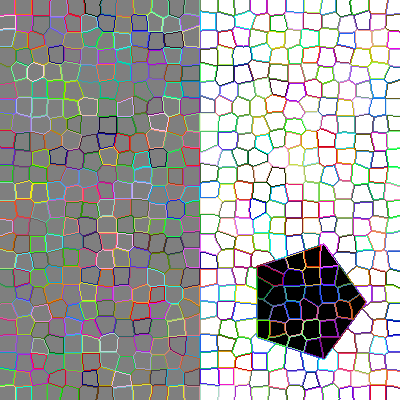
\includegraphics[width = 0.19\textwidth]{inference/1.png}} &
        \fcolorbox{black}{white}{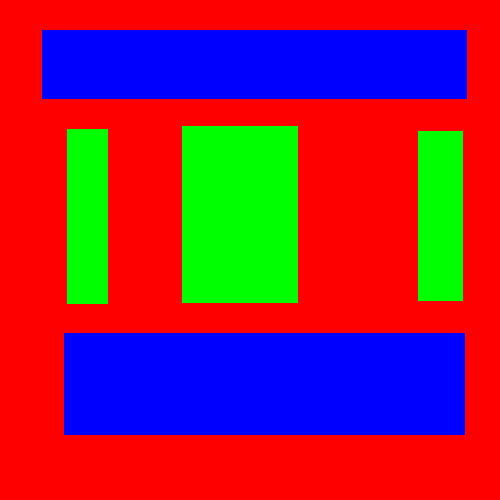
\includegraphics[width = 0.19\textwidth]{inference/2.png}} &
        \fcolorbox{black}{white}{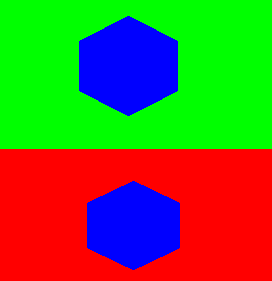
\includegraphics[width = 0.19\textwidth]{inference/3.png}} &
        \fcolorbox{black}{white}{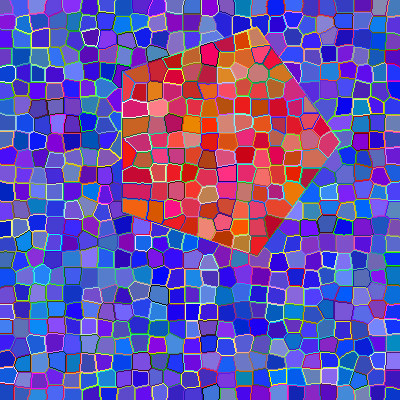
\includegraphics[width = 0.19\textwidth]{inference/4.png}} &
        \fcolorbox{black}{white}{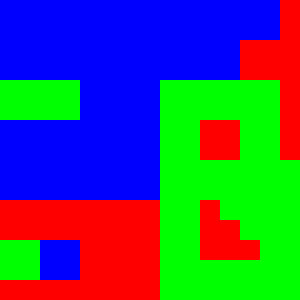
\includegraphics[width = 0.19\textwidth]{inference/5.png}} \\
        \thead{iteration 24} & \thead{iteration 25} & \thead{iteration 26} & \thead{iteration 27} & \thead{iteration 28} \\
        \fcolorbox{black}{white}{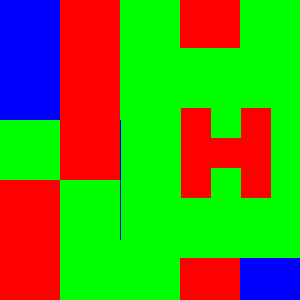
\includegraphics[width = 0.19\textwidth]{inference/24.png}} &
        \fcolorbox{black}{white}{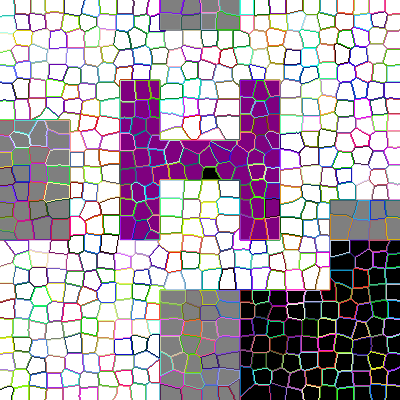
\includegraphics[width = 0.19\textwidth]{inference/25.png}} &
        \fcolorbox{black}{white}{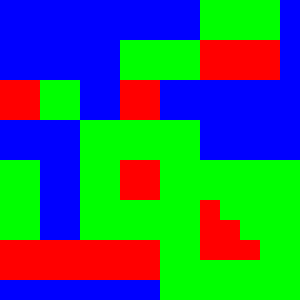
\includegraphics[width = 0.19\textwidth]{inference/26.png}} &
        \fcolorbox{black}{white}{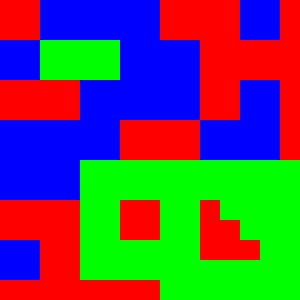
\includegraphics[width = 0.19\textwidth]{inference/27.png}} &
        \fcolorbox{black}{white}{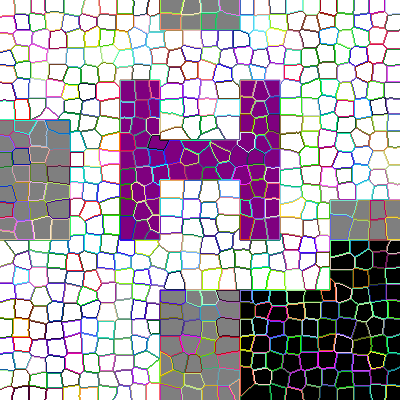
\includegraphics[width = 0.19\textwidth]{inference/28.png}}
    \end{tabular}
    \caption{Inference steps for a sample noised image.}
    \label{fig:inference_example}
\end{figure}

As in case of the noise-free images, in this experiment there was also a slight problem with distinction between label 0 and 3 for narrow and vertical, red stripes that are in the green neighbourhood. Furthermore, for some noised superpixels that were on the object or image boundaries even the pairwise potential did not manage to correct the wrong labelling obtained by the unary potential. Tough the final accuracy of semantic segmentation on images with objects of different shapes was still good. This accuracy expressed as Intersection over Union is presented in Table \ref{table:iou_nonlinear_noised}. Due to the addition of noise the precision of the method is slightly smaller than in previous experiment. The method obtained a mean IoU of 98.39\% for noised images, which is 1.15 percent points lower than in a noise-free case. Segmentation of green and blue regions was correct in 99.93\% and 99.42\% cases respectively. When it comes to red regions, it was 97.92\% for label 0, and 96.27\% for label 3, which is the lowest precision from all classes, just like in case of noise-free images. In this experiment, addition of the pairwise potential improved the final segmentation results to a larger extend than in case of noise-free data. The largest improvement was for objects with a shape of letter H. With the local potential only the accuracy of segmentation into class 3 had the IoU of 90.55\%, which was improved by 5.72 percent points after addition of the pairwise potential. Overally, by using the both potentials to define the energy function segmentation results were more precise by 2.41 percent point comparing to the classification based on local potential only.
\begin{table}[ht]
\centering
\caption{Accuracy of segmentation based on shape detection for noised data.}
\label{table:iou_nonlinear_noised}
    \begin{tabular}{|
    >{\columncolor[HTML]{9B9B9B}}c|c|c|c|c|
    >{\columncolor[HTML]{343434}}c|}
    \hline
    \textit{class} & \cellcolor[HTML]{9B9B9B}label 0 & \cellcolor[HTML]{9B9B9B}label 1 & \cellcolor[HTML]{9B9B9B}label 2 &  \cellcolor[HTML]{9B9B9B}label 3 & {\color[HTML]{FFFFFF} mIoU {[}\%{]}} \\ \hline
    local potential IoU {[}\%{]} & 95.95 & 99.21 & 98.21 & 90.55 & {\color[HTML]{FFFFFF} 95.98} \\ \hline
    final IoU {[}\%{]} & 97.92 & 99.93 & 99.42 & 96.27 &{\color[HTML]{FFFFFF} 98.39} \\ \hline
    \end{tabular}
\end{table}



